\label{1.2.9}

\textit{Projective Closure of an Affine Variety}. If $Y \subseteq \A^n$ is an affine variety, we identify $\A^n$ with an open set $U_0 \subseteq \P^n$ by the homeomorphism $\varphi_0$. Then we can speak of $\overline{Y}$, the closure of $Y$ in $\P^n$, which is called the \textit{projective closure} of Y.

\begin{enumerate}[label = (\alph*)]
    \item Show that $I(Y)$ is the ideal generated by $\beta[J(Y)]$, using the notation of the proof of \cite[2.2]{hartshorne}.
    
    \item Let $Y \subseteq \A^3$ be the twisted cubic of (Ex. \ref{1.1.2}). Its projective closure $\overline{Y} \subseteq \P^3$ is called the twisted cubic curve in $\P^3$. Find generators for $J(Y)$ and $I(\overline Y)$, and use this example to show that if $f_1, \dots, f_r$ generate $J(Y)$, then $\beta(f_1), \dots, \beta(f_r)$ do \textit{not} necessarily generate $I(\overline{Y})$.
\end{enumerate}

\begin{proof}
    \begin{enumerate}[label= (\alph*)]
        \item First and foremost, observe that $I(\overline Y) = I(Z(I(Y))) = \sqrt(I(Y)) = I(Y)$. Hence, we will focus our attention on $I(Y)$.
        
        Recall the definition of $\beta(f) = \beta_0(f) = x_0^d f\parens{\frac{x_1}{x_0}, \dots, \frac{x_n}{x_0}}$ where $d = \deg f$. Let $f \in J(Y)$. Then for all $[a_0 : \dots : a_n] \in Y$ (by which we mean $\phi^{-1}[Y]$), $0=f(\phi([a_0 : \dots : a_n])) = f\parens{\frac{a_1}{a_0}, \dots, \frac{a_n}{a_0}}$. Then indeed, $\beta(f) \in I(Y)^h$. This yields the easier inclusion $(\beta[J(Y)]) \subseteq I(Y)$.

        On the other hand, let $f \in I(Y)^h$. Then for all $\phi^{-1}(a_1, \dots, a_n) = [1 : a_1 : \dots : a_n]$, $f([1 : a_1 : \dots : a_n])$. Letting $\alpha(f) = \alpha_0(f) = f(1, x_1, \dots, x_n)$ this says that $\alpha(f) \in J(Y)$. Naively, we'd just apply $\beta$ and go home, but tragically this fails. Indeed, consider $\beta(\alpha(x_0^d)) = \beta(1) = 1$. $\alpha$ has the potential to lose the data of the $x_0$, but all hope is not lost. Consider $\beta(\alpha(x_0 + x_1)) = \beta(1 + x_1) = x_0 + x_1$, so the issue seems to be with powers of $x_0$. Wih that in mind, let $x_0^e \mid\mid f$ and write $f = x_0^e g$. Then $\alpha(g) = \alpha(f)$, so we'll try to compute $\beta(\alpha(g))$.

        Indeed, $\alpha(g) = g(1, x_1, \dots, x_n)$ so $\beta(\alpha(g)) = g\parens{1, \frac{x_1}{x_0}, \dots, \frac{x_n}{x_0}} x_0^d$. Here, $d = \deg \alpha(g)$ As $f$ is homogeneous and $g = \frac{f}{x_0^e}$, $g$ is homogeneous as well. Thus, if it were the case that $\deg g = d$ then this would be precisely $g$. Indeed, as $x_0 \nmid g$ there must be some monomial summand of $g$ which has no $x_0$ term. This term has the same degree as $g$, as $g$ is homogeneous. Furthermore, applying $\alpha$ to such a term leaves it unchanged. As $\alpha$ cannot increase degree, this means that the degree of $\alpha(g)$ is indeed equal to the degree of $g$, so $g = \beta(\alpha(g))$.

        As discussed, this means that $g = \beta(\alpha(g)) = \beta(\alpha(g)) \in \beta[J(Y)]$. Hence, $f = x_0^e g \in (\beta[J(Y)])$, so $I(Y)^h \subseteq (\beta[J(Y)]) \subseteq I(Y)$. As $I(Y)$ is homogeneous, we get the desired equality $I(Y) = (\beta[J(Y)])$.

        \item The twisted cubic was defined by $Y = \curly{(t, t^2, t^3) : t \in k} \subseteq \A^3$. As shown in \ref{1.1.2}, $Z$ is a variety with ideal $I(Y) = (x_3^3 - x_1, x_2^2 - x_1)$. Applying $\beta$ to these yields $x_3^3 - x_0^2 x_1$ and $x_2^2 - x_0 x_1$. We therefore seek to prove that $I(\overline Y) > (x_3^3 - x_0^2 x_1, x_2^2 - x_0 x_1)$.

        It'd be nice to get some kind of picture here, so in \ref{fig1.2.1} below we show a plot of the twisted cubic curve in affine space.

        \begin{figure}
            \centering
            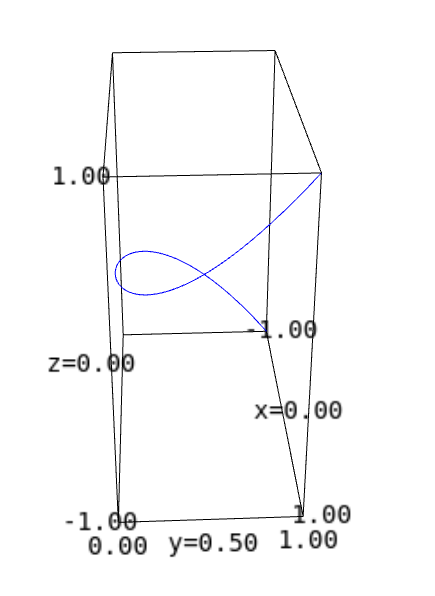
\includegraphics{twisted-cubic-affine}
            \caption{The twisted cubic in $\A^3$}
            \label{fig1.2.1}
        \end{figure}

        Now let's try to visualize this in $\P^3$. We'll appeal to the usual CW complex structure on $\rp^n$. Indeed, we consider $\P^3$ to be the unit ball in $\R^3$ where the boundary sphere has the usual antipoal gluing. If we scale the plot above into the open unit disk, then we get \ref{fig1.2.2}

        \begin{figure}
            \centering
            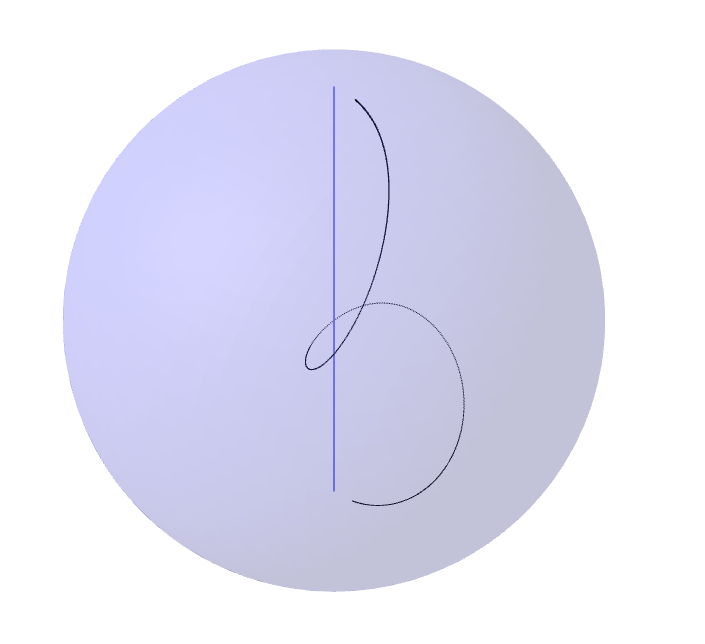
\includegraphics{twisted-cubic-projective}
            \caption{The twisted cubic in $\P^3$}
            \label{fig1.2.2}
        \end{figure}

        This suggests that the closure in $\P^3$ should be the affine twisted cubic along with this blue line $[0 : 0 : 0 :1]$, and that this line is approached by the affine twisted cubic as one ``tends to infinity." How do we make rigorous this idea of tending to infinity? Well the twisted cubic is parametrized by $\A^1$, so it stands to reason that to parametrize its projective closure, and hence to ``tend to infinity" that we would want a parametrization by $\P^1$. Indeed, the affine parametrization is given by $t \mapsto (t, t^2, t^3)$. We'll homogenenize this to get a map $\P^1 \longrightarrow \P^3$ via $[t_0 : t_1] \mapsto [t_0^3 : t_0^2 t_1 : t_0 t_1^2 : t_1^3]$. Restricting to $t_0 = 1$ gives us the original affine parametrization, and the point at infinity $[0 : 1]$ maps to $[0 : 0 : 0 : 1]$ as we expected.

        We claim therefore that the image of this map $\P^1 \longrightarrow \P^3$ (see \ref{1.2.12} for the general case!) is the projective closure of $Y$. Observe that the image of this map is contained in $Z(x_0^2 x_3 - x_1^3, x_0 x_2 - x_1^2, x_0 x_3 - x_1 x_2)$. If we intersect this algebraic set with $x_0 = 1$ we get $Y$ back. If we consider $x_0 = 0$ then these equations yield $x_1^3 = x_1^2 = x_1 x_2 = 0$, which leaves only $[0 : 0 : 0 :1]$. As our intuition suggested, we therefore expect that $\P^1 \longrightarrow \P^3$ has image $Z(x_0^2 x_3 - x_1^3, x_0 x_2 - x_1^2, x_0 x_3 - x_1 x_2) = Y \cup \curly{[0 : 0 : 0 : 1]}$ and that this is precisely $\overline Y$. Indeed, we can do this same trick of considering $t_0 = 1$ and $t_0 = 0$ to prove that this is indeed the image, so it suffices to show that $\overline Y = Y \cup \curly{[0 : 0 : 0 :1]}$.

        Certainly $Y \cup \curly{[0 : 0 : 0 : 1]}$ is closed. Thus, if $Y$ itself is not closed then certainly this must be the closure. If $Y$ was closed, then $Y \cup \curly{[0 : 0 : 0 : 1]} = Z(x_0^2 x_3 - x_1^3, x_0 x_2 - x_1^2, x_0 x_3 - x_1 x_2)$ seperates this closed set into two disjoint closed sets. However, it is not hard to see that our map $\P^1 \longrightarrow \P^3$ is continuous, and $\P^1$ is connected, so the image must be connected as well. Thus, this decomposition would be a contradiction so $Y$ is not closed. Hence, we have computed $\overline Y = \im(\P^1 \longrightarrow \P^3) = Z(x_0^2 x_3 - x_1^3, x_0 x_2 - x_1^2, x_0 x_3 - x_1 x_2)$.

        We can finally show that $(x_3^3 - x_0^2 x_1, x_2^2 - x_0 x_1) < I(\overline Y)$. Indeed, $[0 : 0 : 1 : 1] \in Z(x_3^3 - x_0^2 x_1, x_2^2 - x_0 x_1)$ but is not in $\overline Y$, so we have the strict containment.

        However, we are still asked to find actual generators for $I(\overline Y)$. Our best guess is of course $(x_0^2 x_3 - x_1^3, x_0 x_2 - x_1^2, x_0 x_3 - x_1 x_2)$, but we only know that the radical of this ideal is $I(\overline Y)$. There's probably a way to do all this nonsense, but we'll defer it to \ref{1.2.12}. Should that problem remain unsolved, mutter something about Gr\"obner bases to stop worrying about this computation.
    \end{enumerate}
\end{proof}
